The following results are displayed using graphs to highlight some of the insights we have taken from the experiments we ran. Blue line and text represents our simplest crossover that swaps the last halves of two parents to create two children described in(3. X1). The red represents the second crossover that selects genes from each parent based on their fitness scores, described in (3. X2). The orange represents the third crossover that selects contiguous segments of genes from each parent based on their fitness scores, described in (3. X3).

We started of with a fitness function that gave 10 points for each person served, which in the end promoted the algorithm to serve all people in the building. The problem with this was that it tended to give long genomes because it was more beneficial to serve all people than to serve them quickly. We then changed fitness function to one that gave huge penalties for all people that wasn't served by the elevator when the route was finished. It also increased the score with one for each person not arriving to its destination for each floor traveled. This means that the lower score the better. It also made it possible for us to analyze the average waiting time and this was also a benchmark that most papers we found used for this kind of problem.

\newpage

\subsection{Building 1}
% references here
Figure \ref{fig:Building1 results} shows results with 100 people in the building and the worst performance from 5 runs for each crossover on the smallest building with 10 people in it. Figure \ref{fig:Building1 worst} displays the worst case in these runs where the blue crossover failed to serve one person and then received a huge penalty. We used figure \ref{fig:Building1 100 people} to highlight that with more people inside the orange crossover kept getting good results with great consistency. The blue one also performed as good as the orange one, but it wasn't as consistent. The red one was extremely unreliable it performed well sometimes, but it also got stuck in local minimums for long time periods. Besides that it took more generations for all crossovers to reach an acceptable solution because of the increased number of people. The orange and blue crossover often reached a good solution quicker than the red one, and it also tends to get worse the more people it has to serve.

\begin{figure}[ht]
	\centering
	\begin{subfigure}[b]{0.49\linewidth}
		\centering
		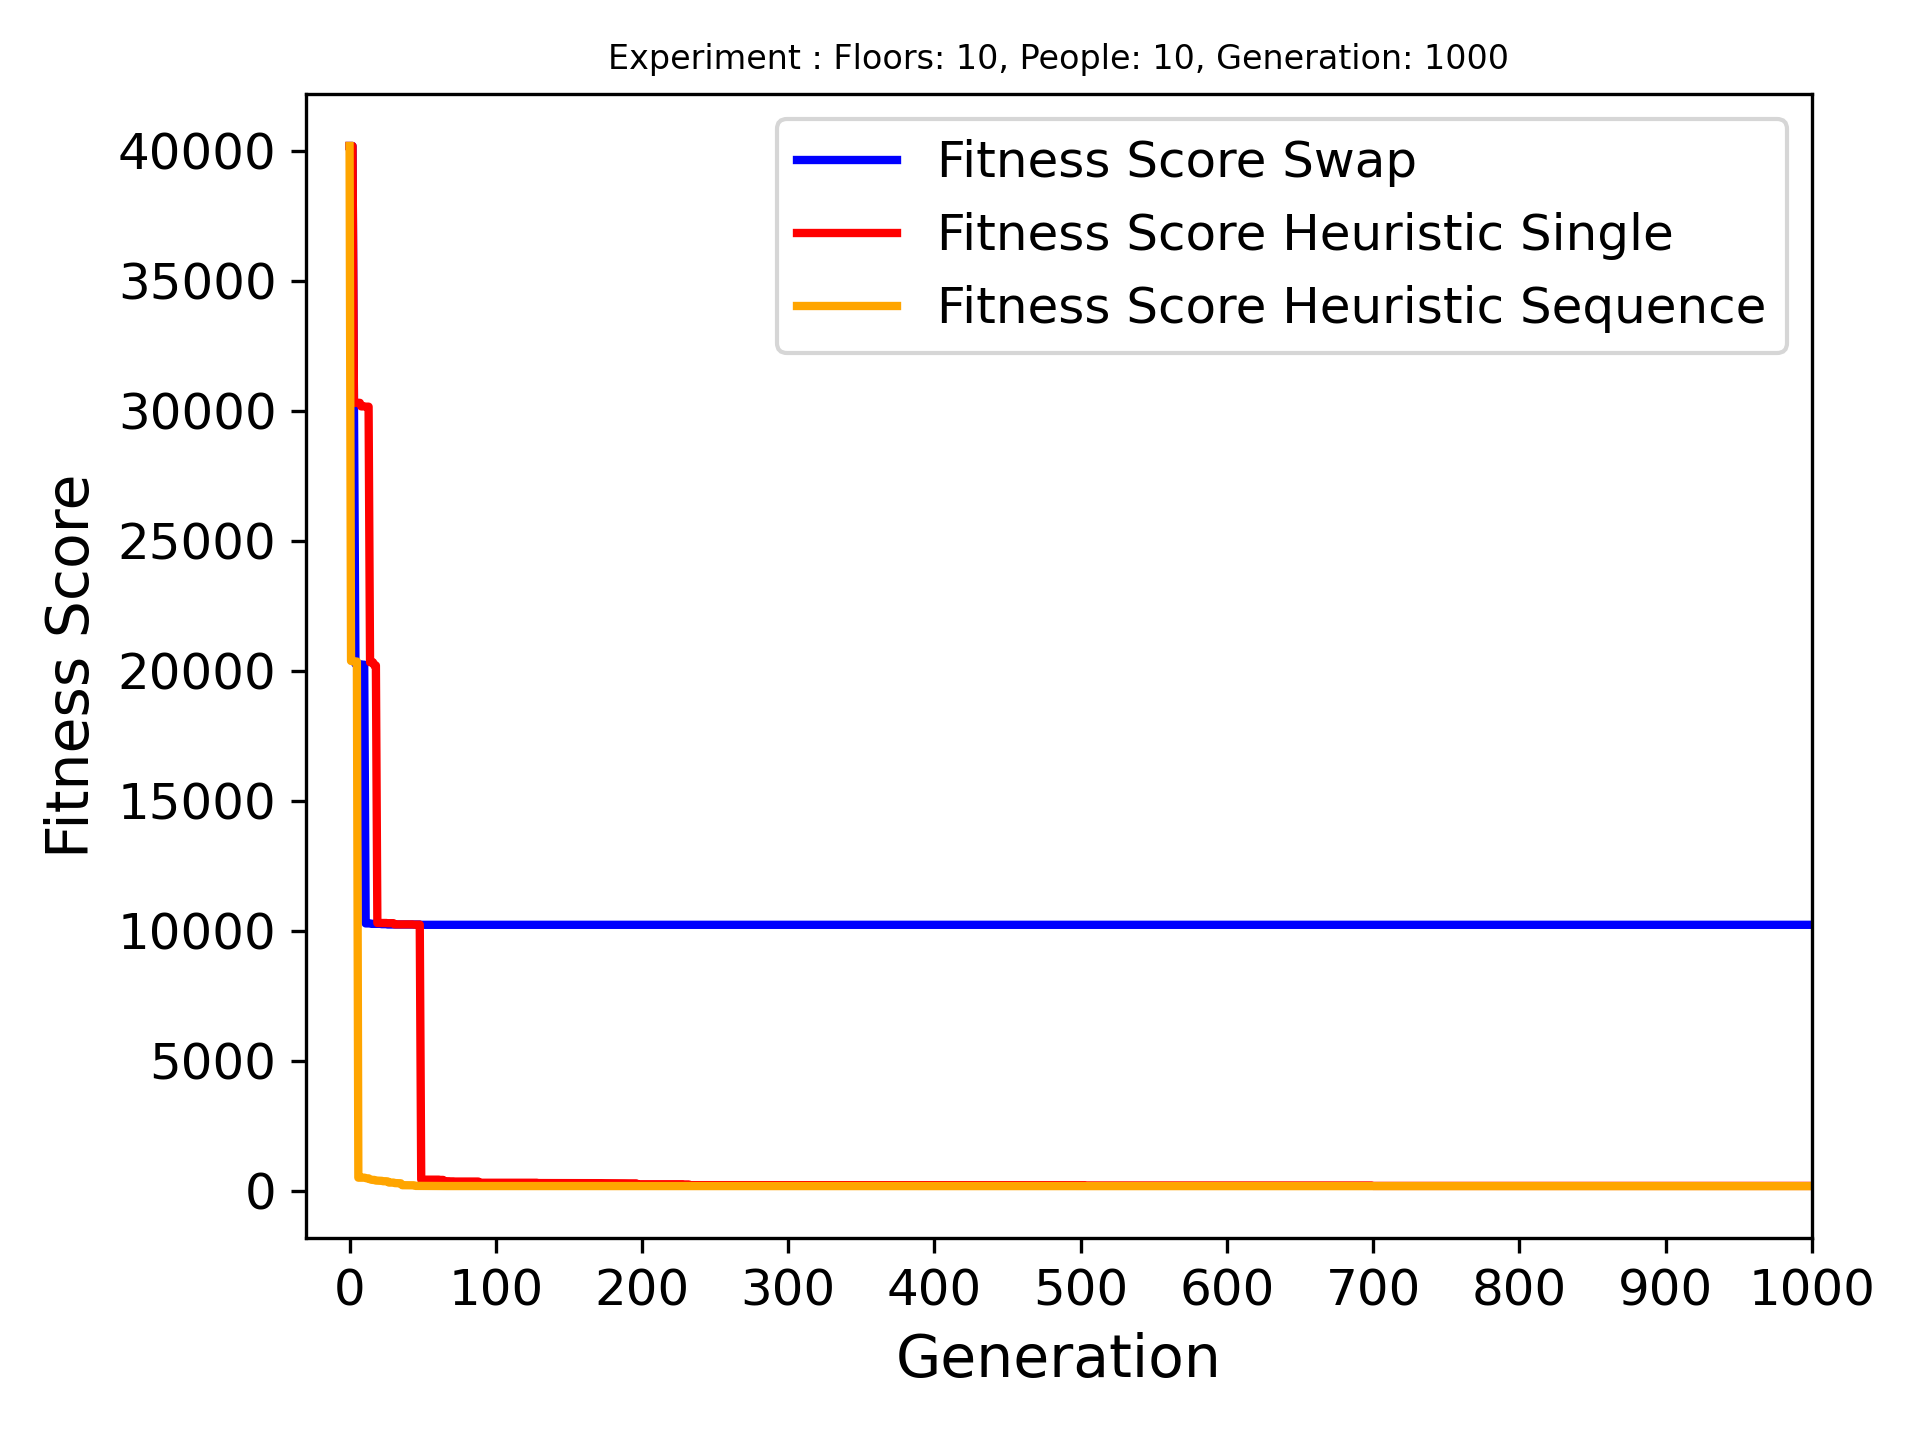
\includegraphics[width=\linewidth]{results/Building1/Mutation_0.1/Floors: 10, People: 10, Generation: 1000_worst.png}
		\captionsetup{justification=centering,font=tiny}
		\caption{Score/Arrived/Length:\\\textcolor{blue}{10227/9/9}, \textcolor{red}{182/10/11}, \textcolor{orange}{172/10/11}.}
		\label{fig:Building1 worst}
	\end{subfigure}
	\hfill
	\begin{subfigure}[b]{0.49\linewidth}
		\centering
		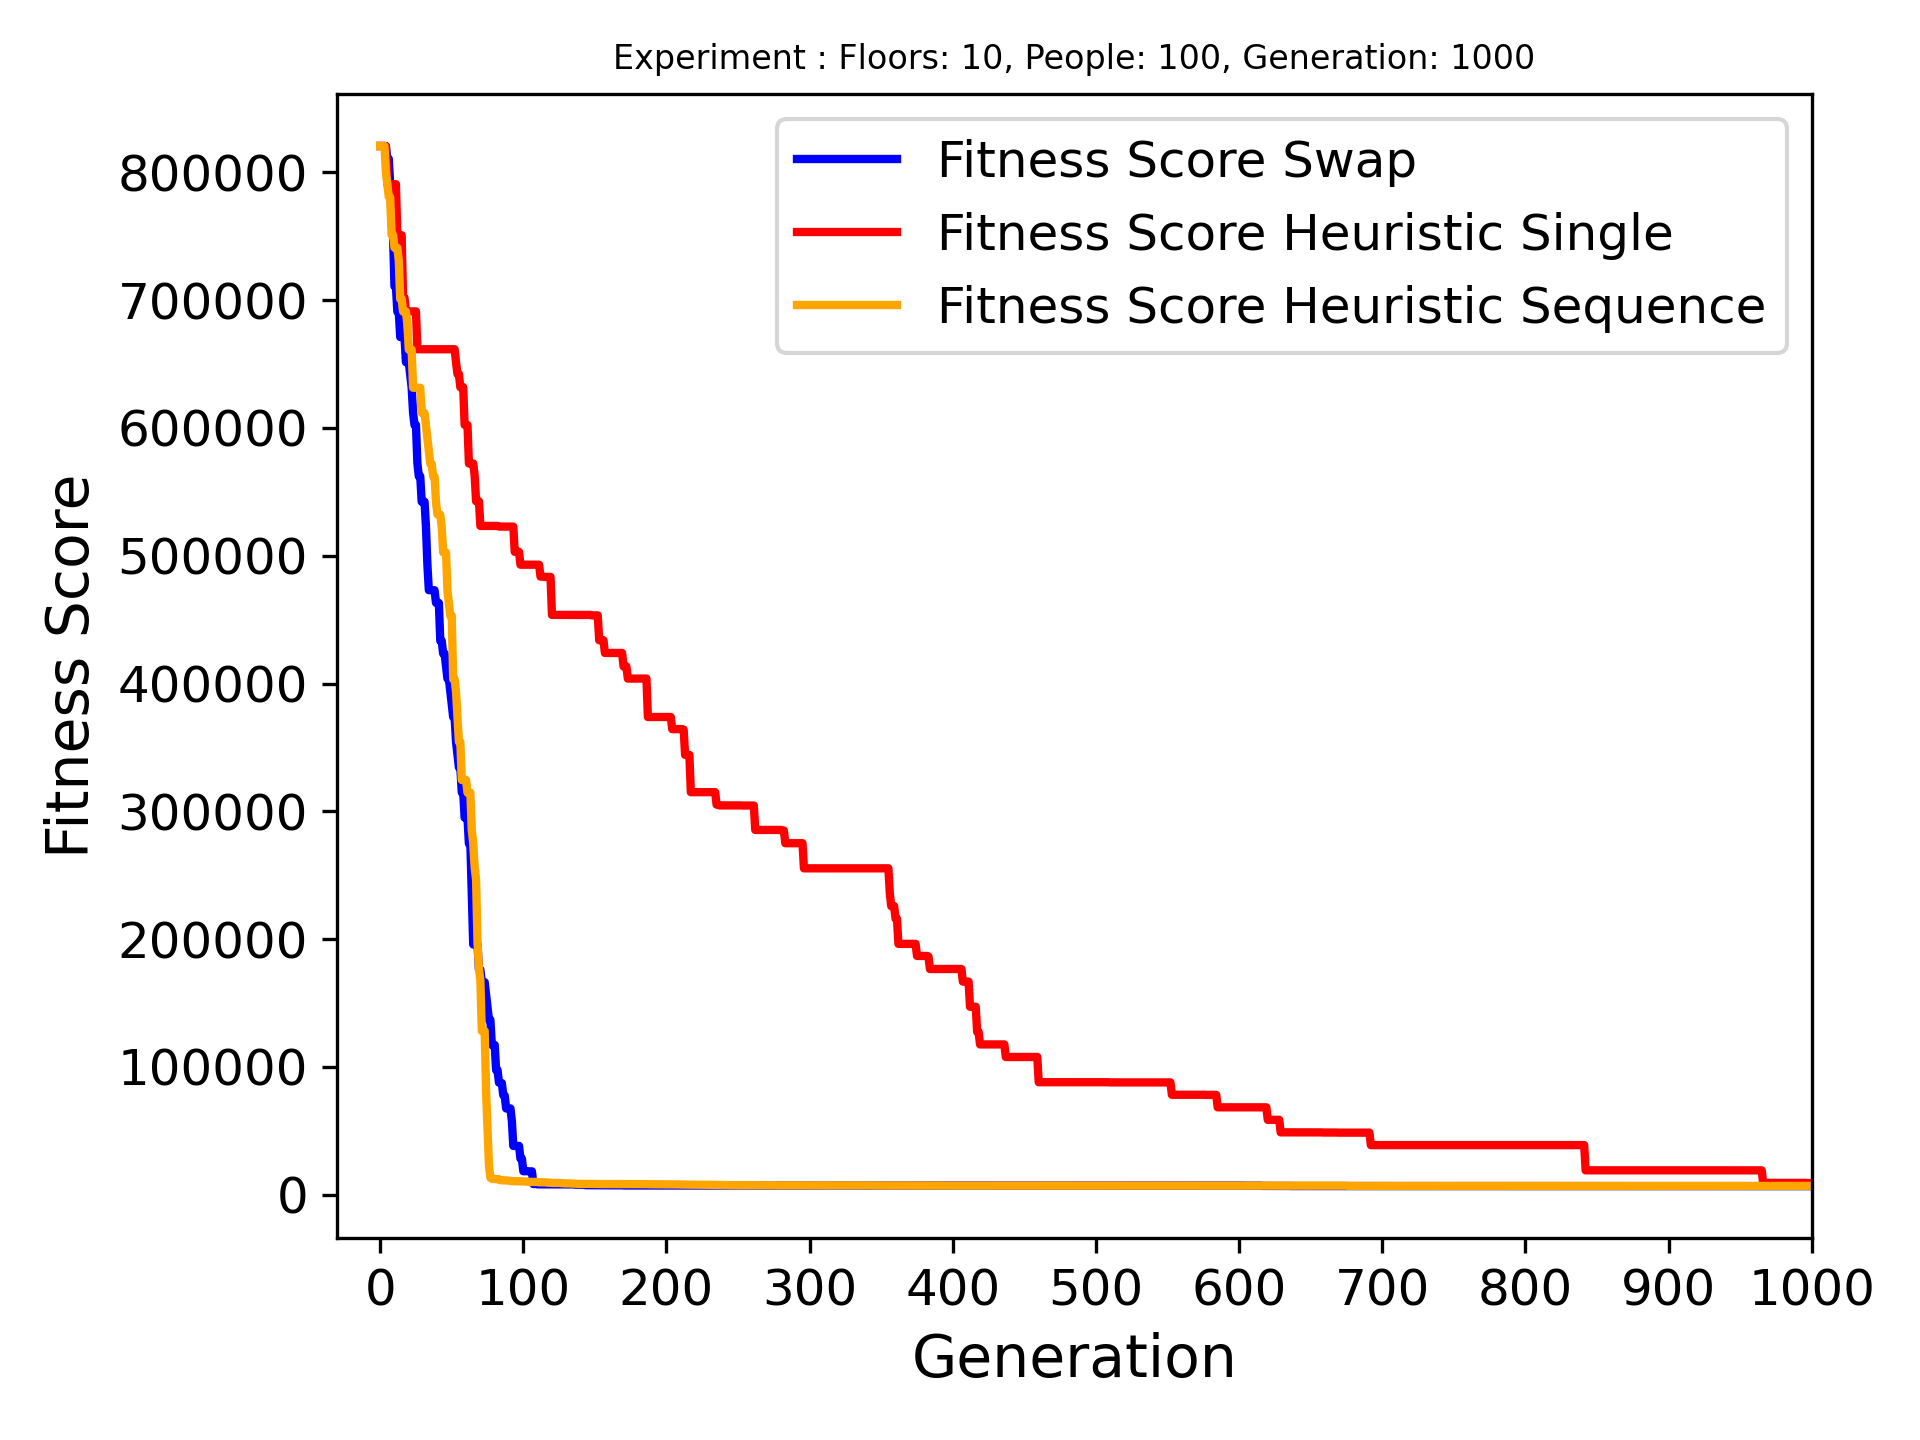
\includegraphics[width=\linewidth]{results/Building1/Mutation_0.1/Floors: 10, People: 100, Generation: 1000.png}
		\captionsetup{justification=centering,font=tiny}
		\caption{Score/Arrived/Length:\\\textcolor{blue}{6727/100/45}, \textcolor{red}{9113/100/61}, \textcolor{orange}{6880/100/52}.}
		\label{fig:Building1 100 people}
	\end{subfigure}
	\captionsetup{font=scriptsize}
	\caption{Building 1 comparing worst and best case.}
	\label{fig:Building1 results}
\end{figure}

\newpage

\subsection{Building 2}
Our second building for experiment is a direct copy from INVESTIGATION OF OPTIMIZATION TECHNIQUES ON THE ELEVATOR DISPATCHING PROBLEM\cote{gharieb2005optimal}. The population has the same starting floor and destination. The parameters for elevator population and number of generations are also set to match the values used for the experimentation in the paper. This was done to get a fair comparison between their results and ours. In their genetic algorithm they are using Davis-order crossover, swap mutation, elitism and their fitness function is calculating the average traveling time for all passengers. It is much like ours but we allow the length of a chromosome to change in the mutation operator. The average result they got from 5 runs was 279.1s per traveler, and the average from our 5 runs was 305.1s. Our algorithm was on average 26s (~8.5\%) slower than the result in the paper. As always this could have been just a coincidence but one factor might have been that Davis-order crossover divides the chromosome into more segments while ours only splits it into two larger segments. Why this might affect the result is because when we split the parent chromosome into two larger segments, parts of them will probably not contribute to a better result and they will have a larger chance for remaining throughout more generations. An approach that would have been interesting to test is to implement elements of heuristic operators into Davis-order crossover. This would allow for more segments being made but also have the more “dominant” parent transfer more of its genes into the next generations.

\newpage

\subsection{Building 3}
As mentioned earlier the red crossover tends to perform worse the more people in the building instances and Figure \ref{fig:Building3 results} highlights this phenom again. In figure \ref{fig:Building3 worst} the blue crossover actually outperform the orange one, that got stuck in a local minimum for a long time. The orange one also was slower than the blue one. In addition, figure \ref{fig:Building3 best} then shows a case where the blue one performed similar to how it performed in \ref{fig:Building3 worst} and the orange one reached an extraordinary low score of 121157 without getting stuck in a local minimum. With other words this pinpoints that the orange crossover have a good worst case and great best case which makes it the most reliable crossover of the three.

\begin{figure}[ht]
	\centering
	\begin{subfigure}[b]{0.49\linewidth}
		\centering
		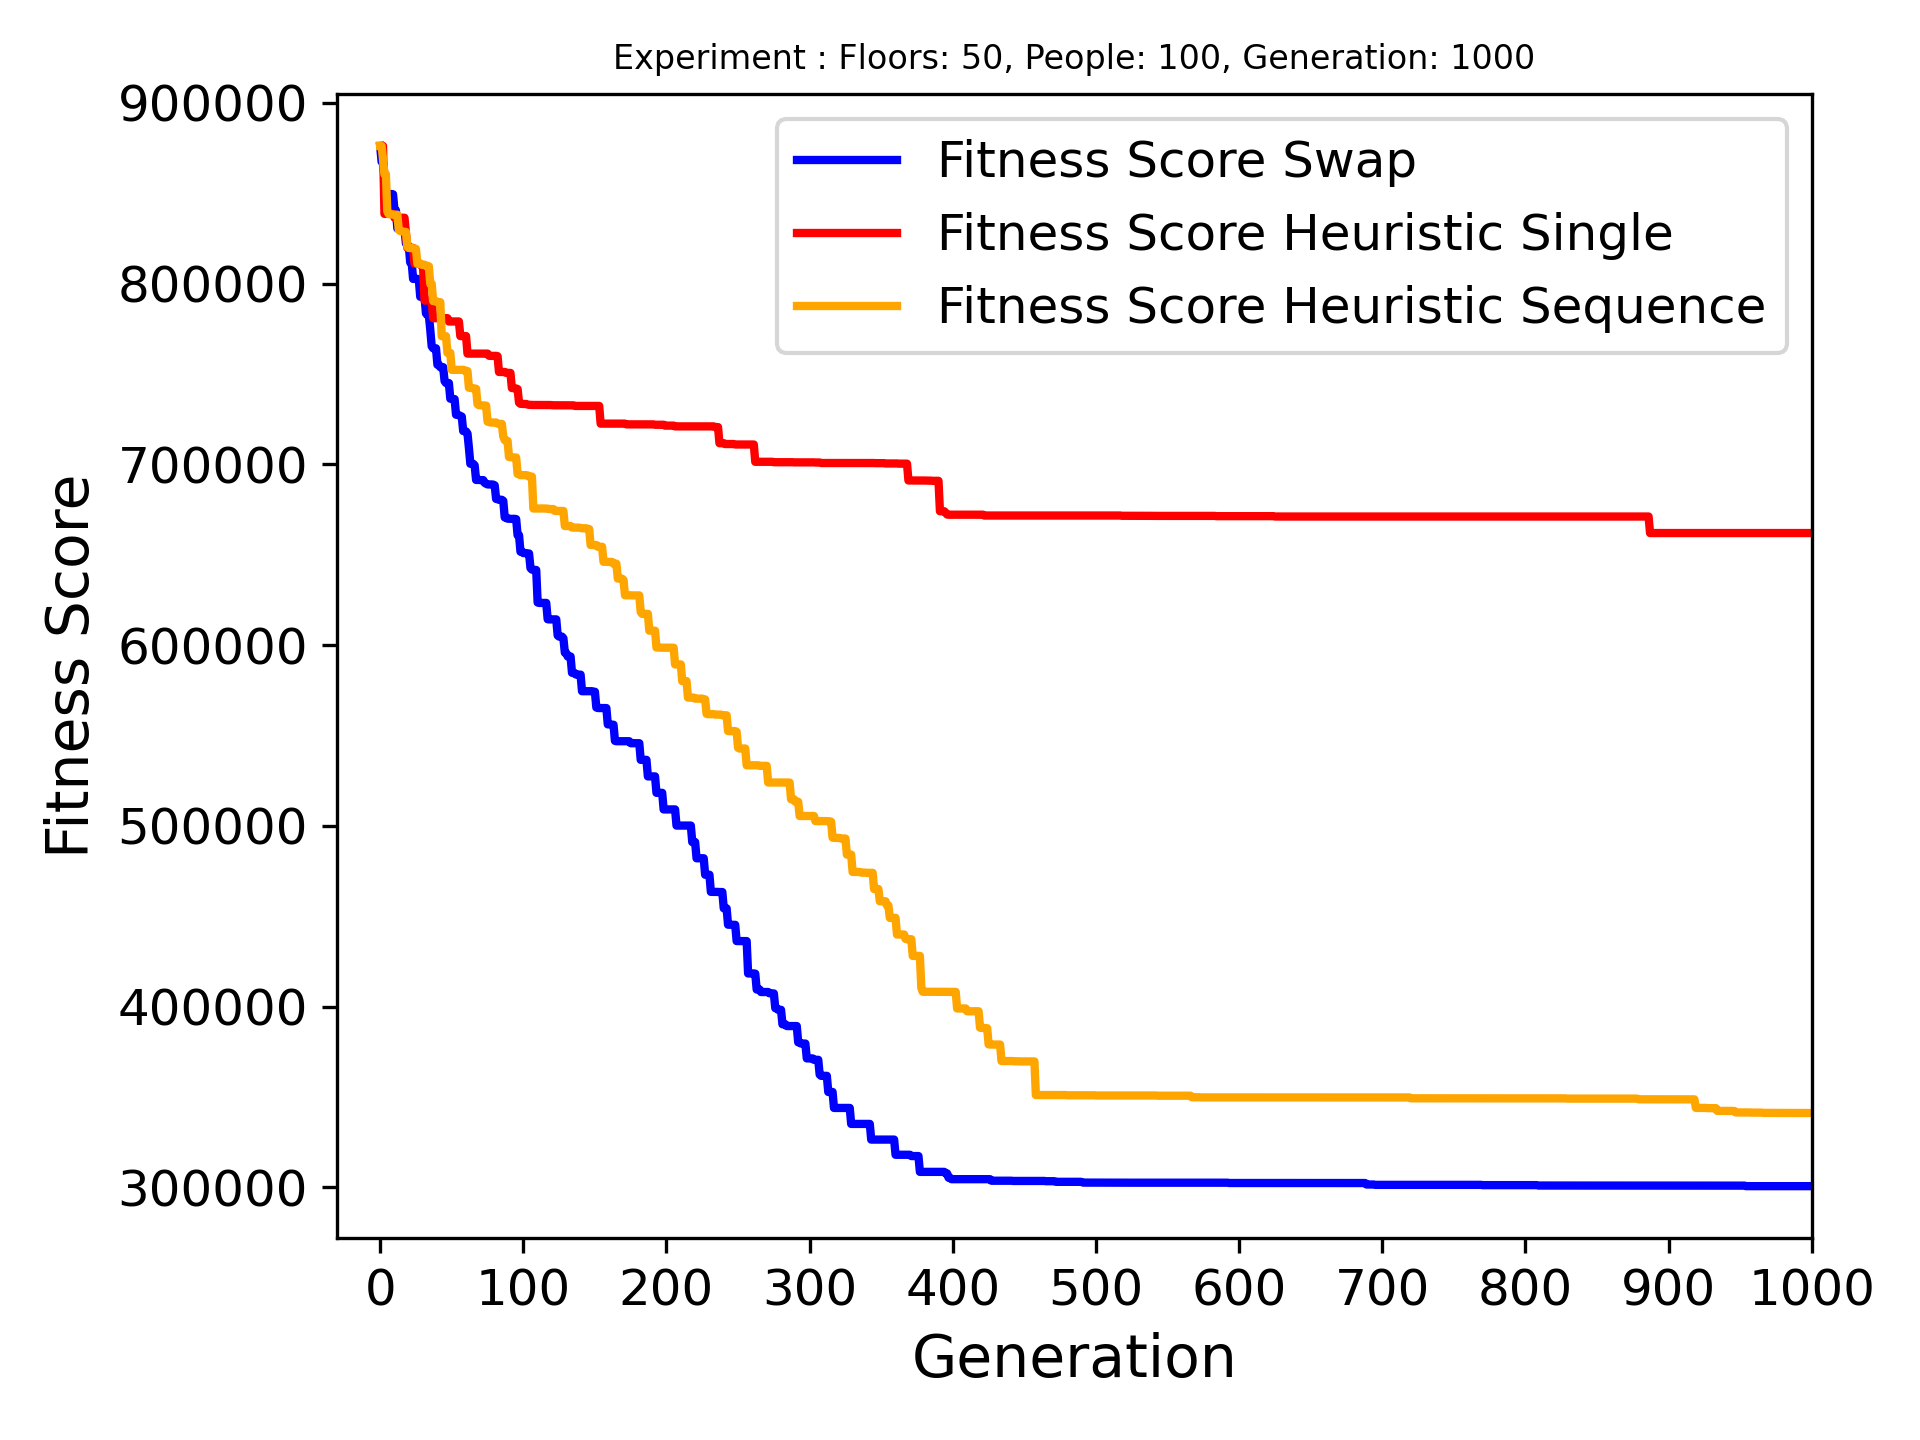
\includegraphics[width=\linewidth]{results/Building3/Mutation_0.1/Floors: 50, People: 100, Generation: 1000_4_worst.png}
		\captionsetup{justification=centering,font=tiny}
		\caption{Score/Arrived/Length:\\\textcolor{blue}{300697/74/69}, \textcolor{red}{661991/35/52}, \textcolor{orange}{341167/69/74}.}
		\label{fig:Building3 worst}
	\end{subfigure}
	\hfill
	\begin{subfigure}[b]{0.49\linewidth}
		\centering
		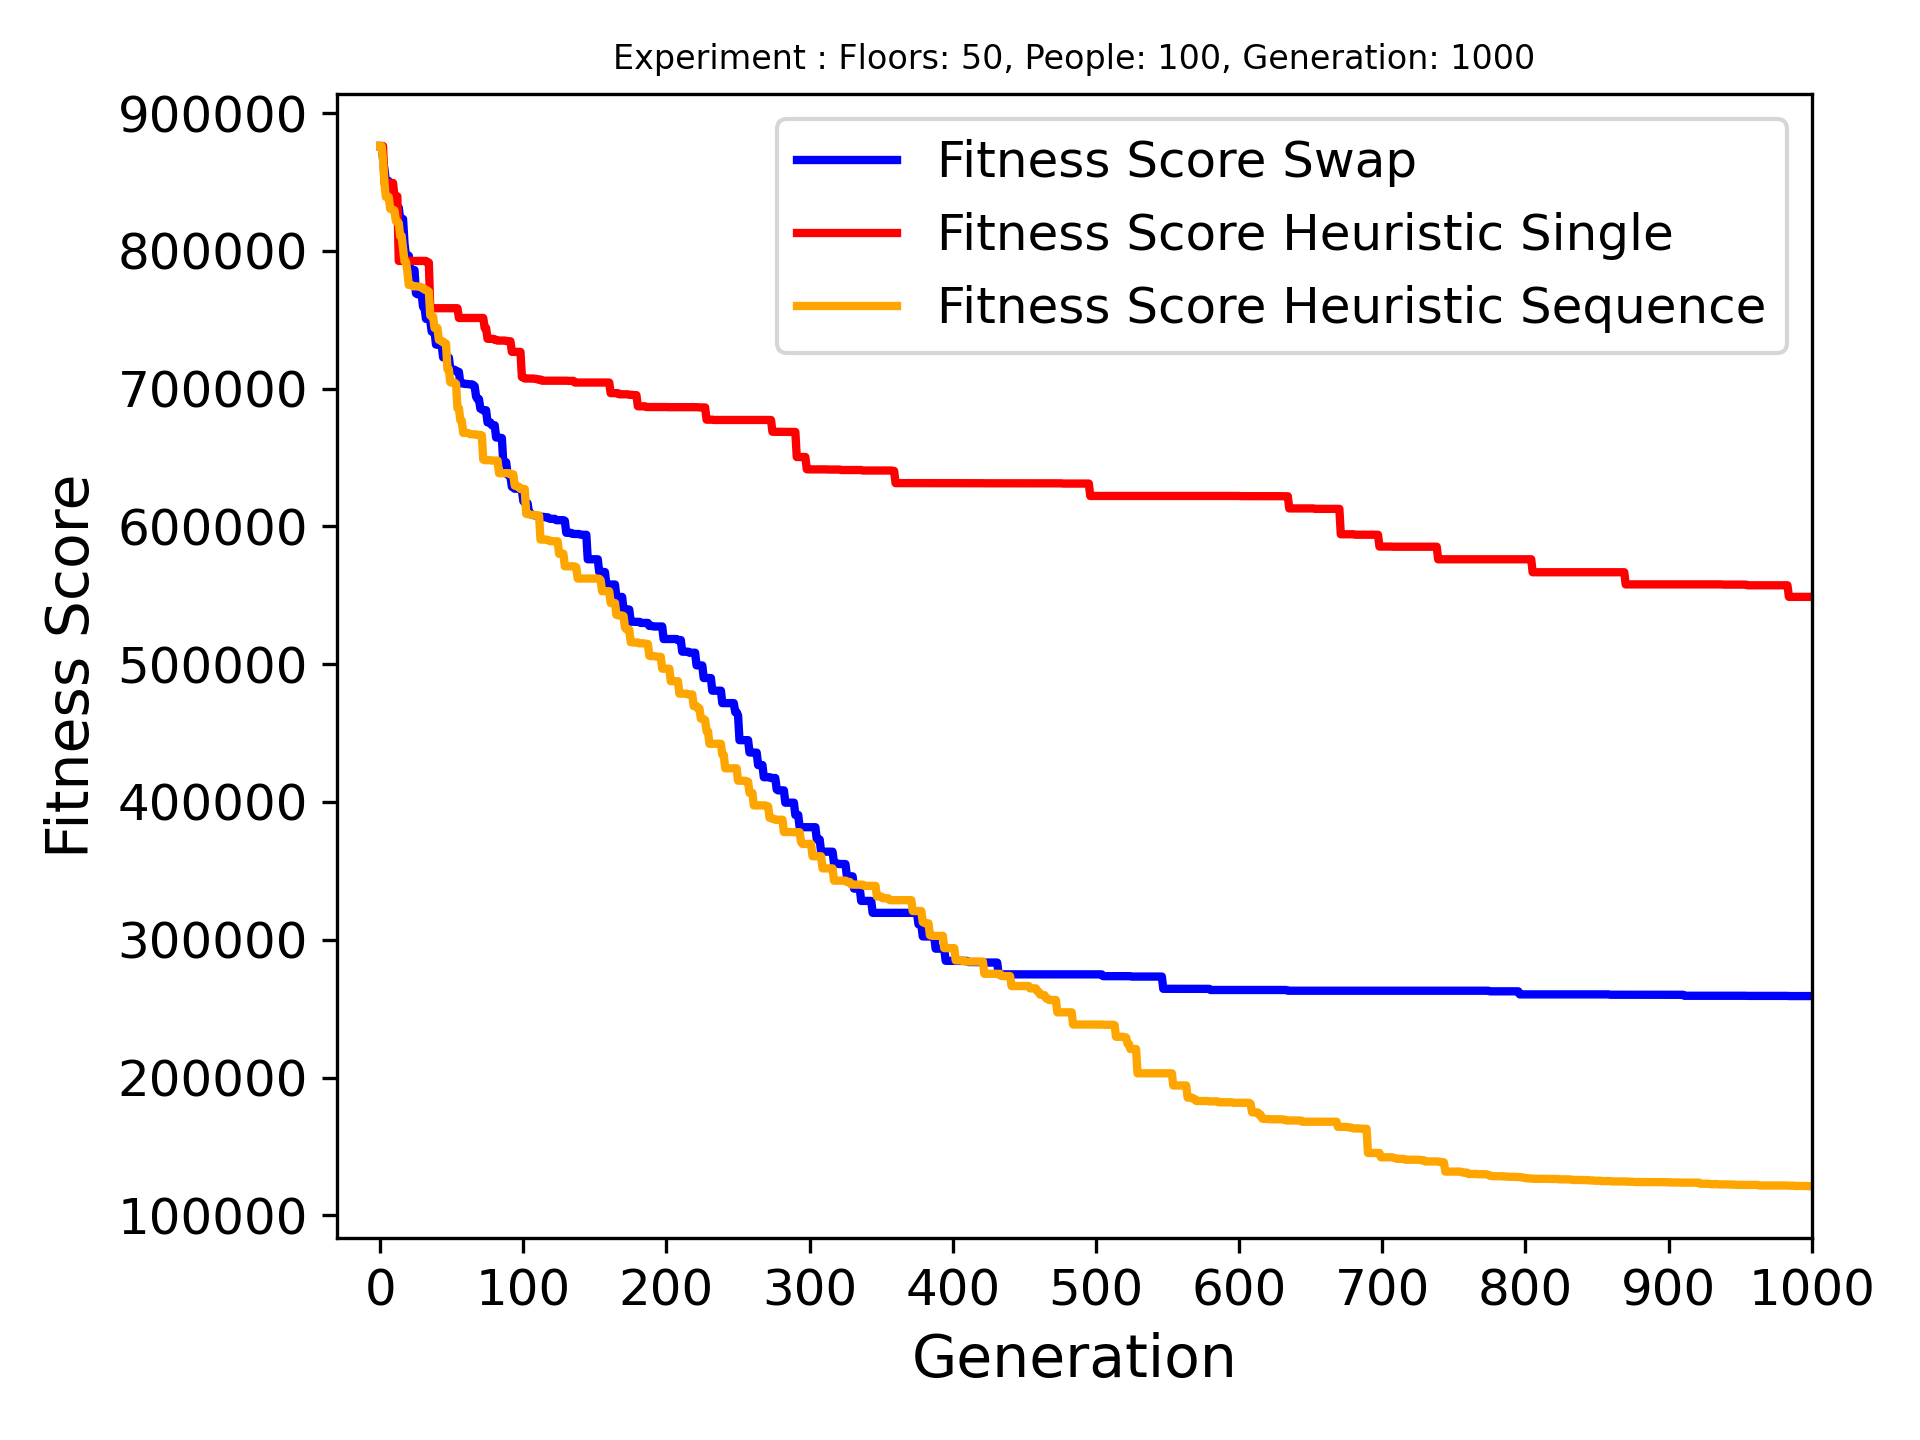
\includegraphics[width=\linewidth]{results/Building3/Mutation_0.1/Floors: 50, People: 100, Generation: 1000_1_best.png}
		\captionsetup{justification=centering,font=tiny}
		\caption{Score/Arrived/Length:\\\textcolor{blue}{259130/79/71}, \textcolor{red}{548857/48/59}, \textcolor{orange}{121157/94/124}.}
		\label{fig:Building3 best}
	\end{subfigure}
	\captionsetup{font=scriptsize}
	\caption{Building 3 comparing worst and best case.}
	\label{fig:Building3 results}
\end{figure}
\newpage
\subsection{Building 4}
After running all the buildings with mutation rate of 10\% we started testing out different values and quickly found out that our algorithm found a solution that serves all or almost all people much faster with a greater mutation rate. We display result from runs with a mutation rate of 60\%. \ref{fig:Building 4 results} shows how much faster our algorithm reach acceptable solutions than before. When mutation rate was low the best solutions gave us fitness scores around 500 000 but with a high rate we were able to get scores around 200 000. The best run served 66 people when mutation was 10\%, the best run with mutation 60\% served all 100 people. Reason behind this is that to be able to serve as many people as possible the genes have to mutate to become longer than number of floors. With a higher mutation rate this happens in much quicker pace and therefore the algorithm is able to leave local minimums faster. Therefore, a greater mutation rate is beneficial and less computational power is needed compared to increasing the population size or the number of generations. We tested increasing number of generations and received similar results as with a greater mutation rate. If we had more time to experiment with different mutation rates we could probably find an even better rate.

\begin{figure}[ht]
	\centering
	\begin{subfigure}[b]{0.49\linewidth}
		\centering
		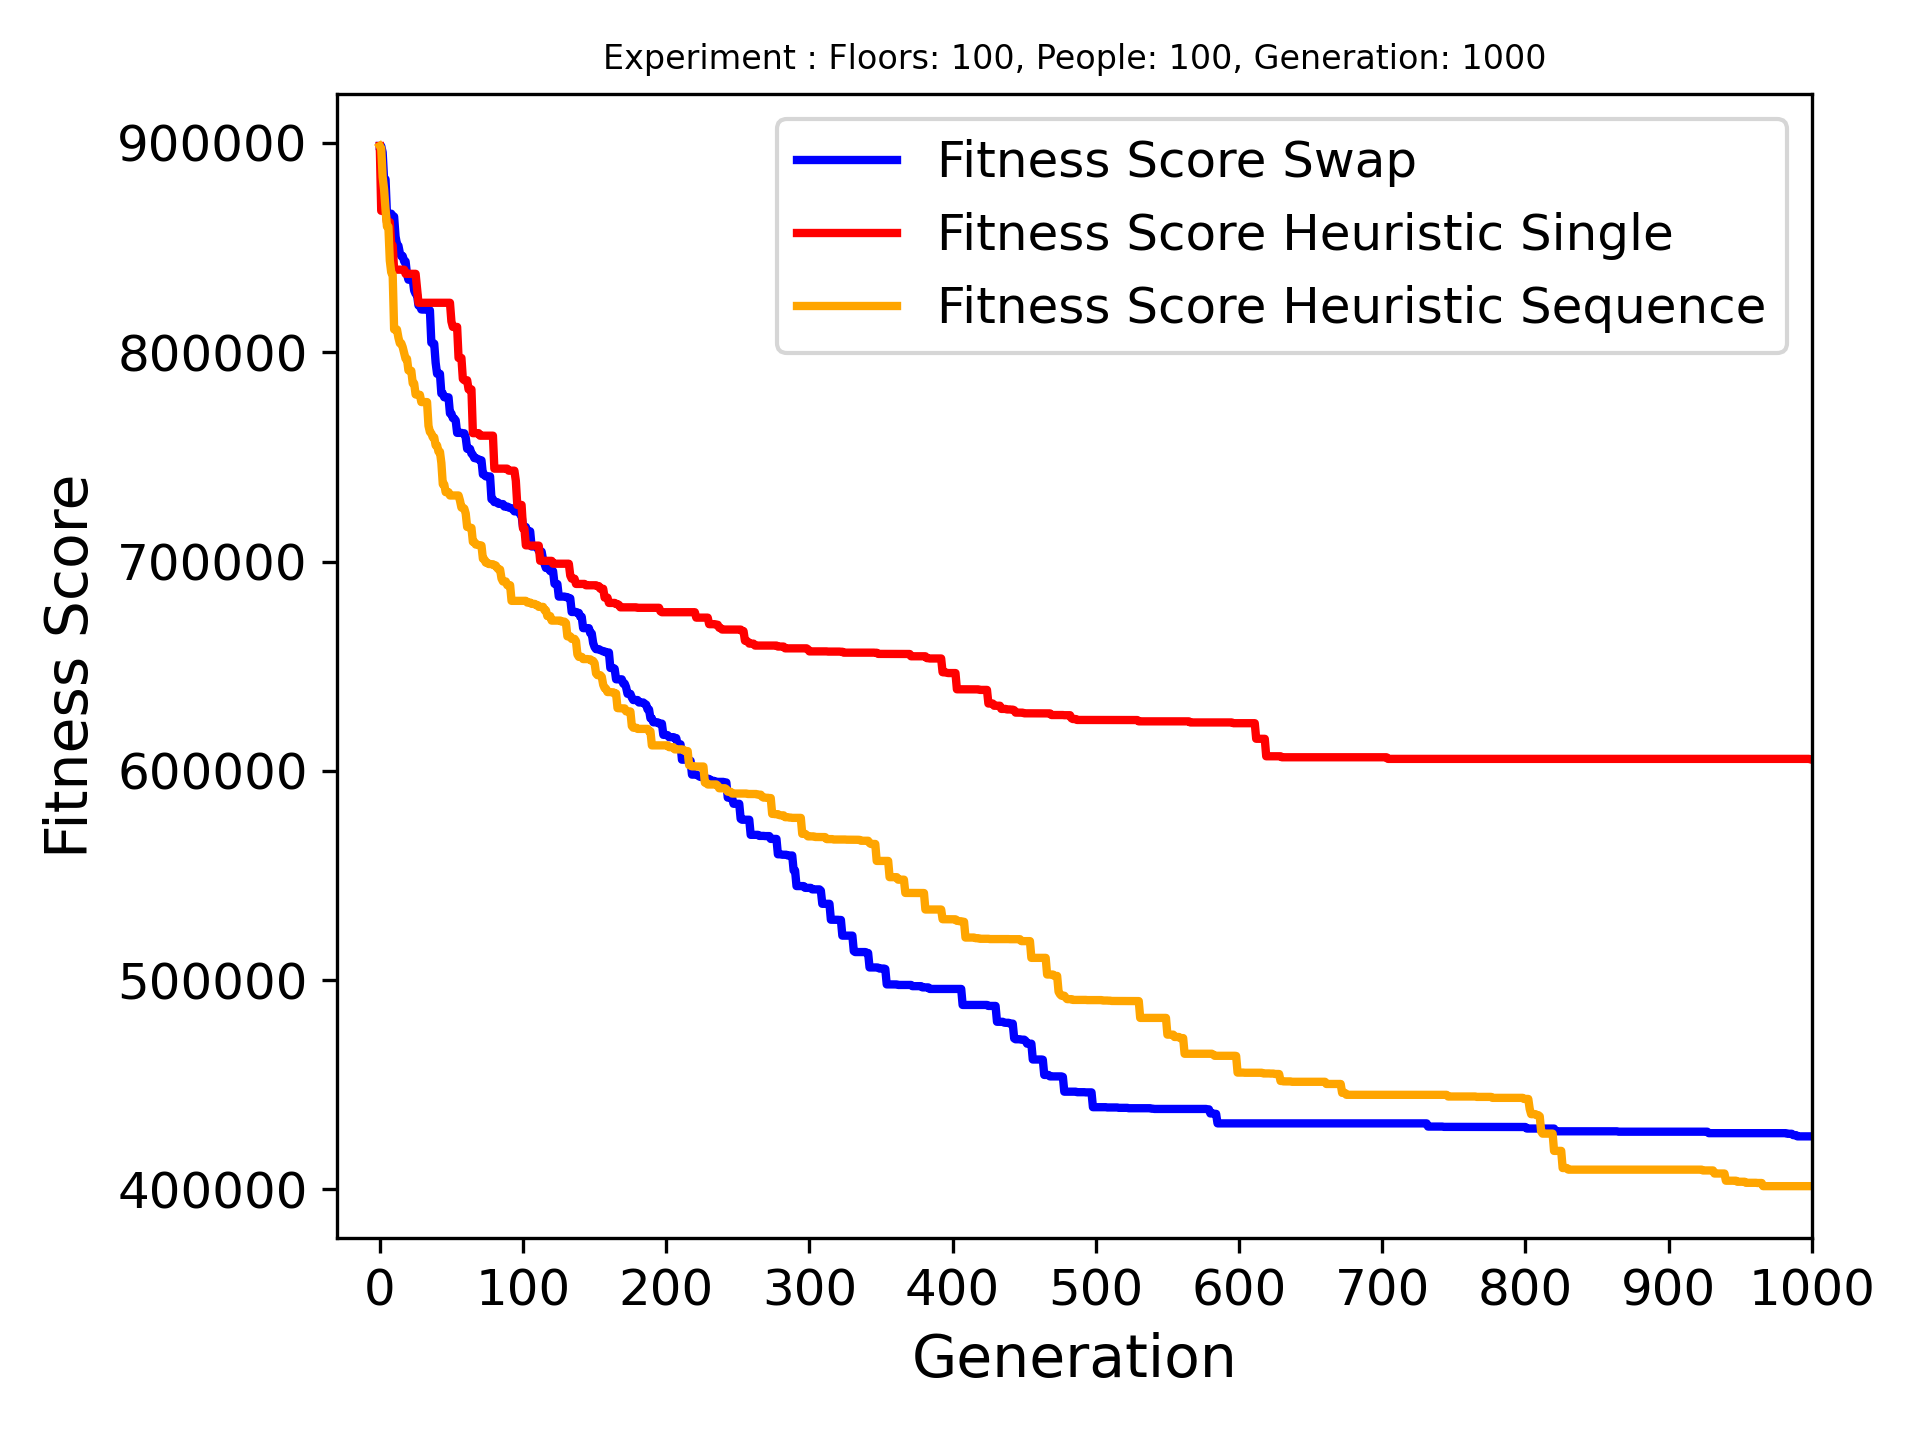
\includegraphics[width=\linewidth]{results/Building4/Mutation_0.1/Floors: 100, People: 100, Generation: 1000_2_best.png}
		\captionsetup{justification=centering,font=tiny}
		\caption{Score/Arrived/Length:\\\textcolor{blue}{425352/67/80}, \textcolor{red}{605508/44/102}, \textcolor{orange}{401562/66/75}.}
		\label{fig:Building4/Mutation_0.1/Floors: 100, People: 100, Generation: 1000_2_best}
	\end{subfigure}
	\hfill
	\begin{subfigure}[b]{0.49\linewidth}
		\centering
		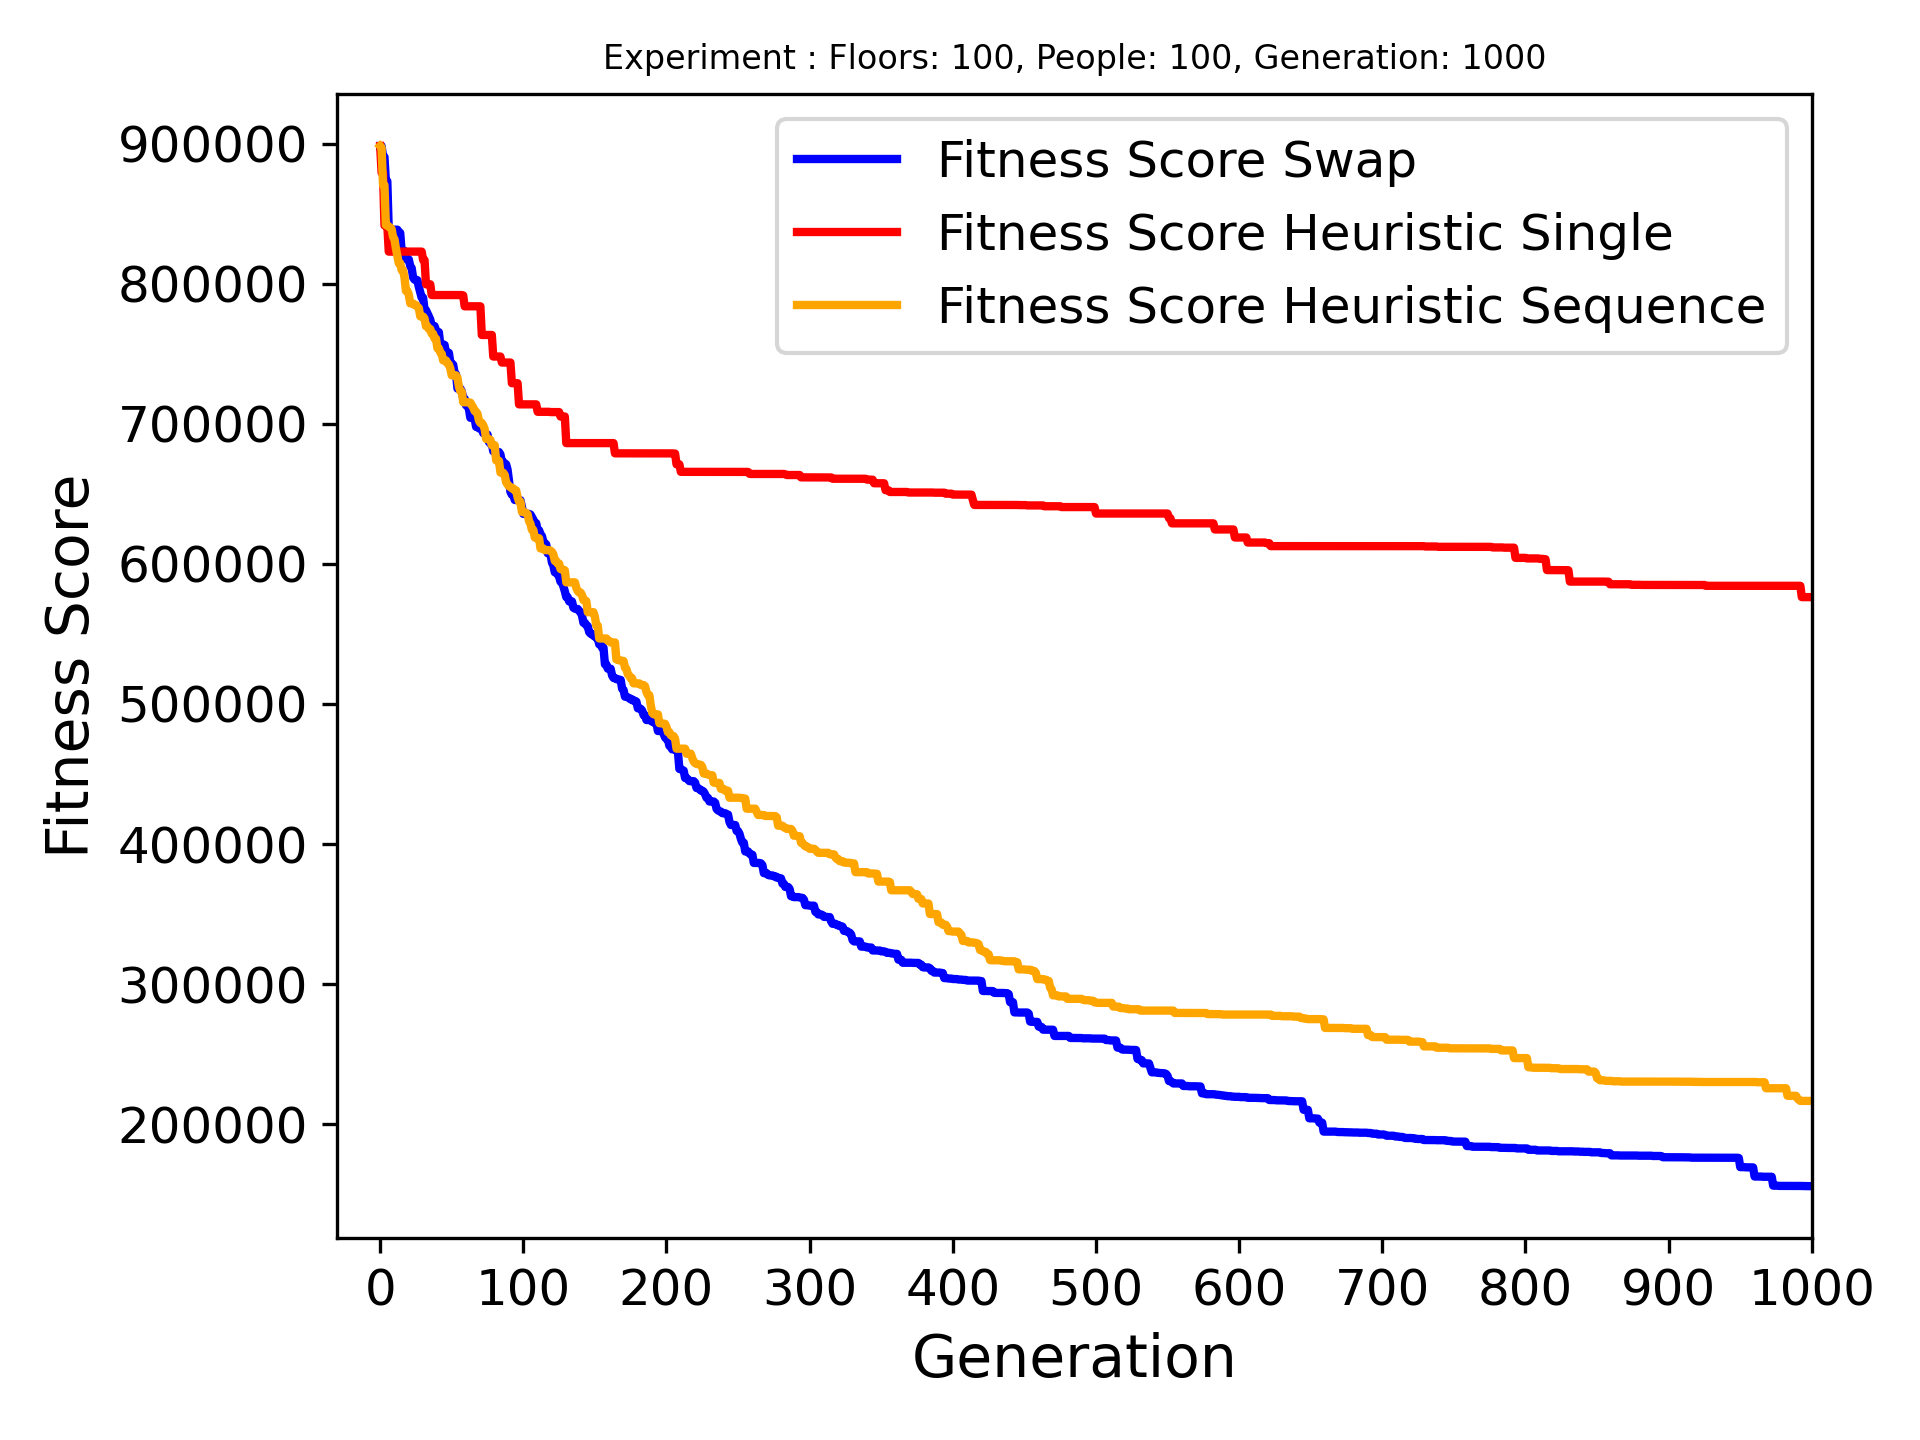
\includegraphics[width=\linewidth]{results/Building4/Mutation_0.6/Floors: 100, People: 100, Generation: 1000_best.png}
		\captionsetup{justification=centering,font=tiny}
		\caption{Score/Arrived/Length:\\\textcolor{blue}{155619/100/151}, \textcolor{red}{576322/48/117}, \textcolor{orange}{216508/94/139}.}
		\label{fig:Building4/Mutation_0.6/Floors: 100, People: 100, Generation: 1000_best}
	\end{subfigure}
	\captionsetup{font=scriptsize}
	\caption{Building 4 comparing different mutation rates.}
	\label{fig:Building 4 results}
\end{figure}

